\chapter{Holographic Video Microscopy}
\label{ch:hvm}

% Suggested figures.
% Diagrams depicting the physical processes
% sequentially.
% The setup.

\newcommand{\einc}{\vec{E}_{\text{inc}}}
\newcommand{\escat}{\vec{E}_{\text{s}}}
\newcommand{\eadd}{\vec{E}_{\text{add}}}
\def\Plus{\texttt{+}}

\section{Overview}

%In this chapter, we will review the salient details 
%underlying the theory and experimental implementation
%of holographic video microscopy. Whenever possible,
%extraneous details that detract from our narrative
%will be relegated to the appendix or be given 
%primary source citations.


%Holographic video microscopy illuminates a sample of scatterers with
%coherent illumination in order to preserve phase information.
Holographic video microscopy (HVM) utilizes coherent
illumination to measure physical properties of micron-sized particles,
primarily their size, refractive index, and three-dimensional position.
By imaging a sample with coherent illumination, the normally averaged-away
phase information is preserved and contributes to the intensity variations
in the resulting image. The physical properties of individual scatterers
are encoded in this phase information and can be extracted by fitting
the resulting intensity patterns to an appropriate light scattering theory.
For non-absorbing dielectric spheres between $\num{1}$-$\SI{10}{\um}$,
this technique yields nanometer-scale precision for the three-dimensional
position and radius, and part-per-thousand precision for the refractive index.

In this chapter, we acquaint the reader with our primary experimental
HVM setup and in so doing outline the salient physical processes underlying
the technique. We then describe the Lorenz-Mie theory of light
scattering, % and discuss the validity of common assumptions.
discuss our implementation of image analysis, and 
conclude with a number of applications of holographic video
microscopy.


\section{Experimental Setup}
\label{ch:hvm:sec:hvm}

A diagram of our custom-built in-line holographic microscope
is provided in Fig.~%\ref{fig:hvm_01}.
Our setup illuminates
the sample plane with a blue ($\SI{447}{nm}$ vacuum wavelength),
linearly polarized laser beam (Coherent Cube). The beam's
$\SI{25}{\mW}$ of power is spread over the $\SI{3}{\mm}$ beam
diameter, producing an average irradiance of approximately
$\SI{0.88}{\mW / \mm^2}$. Before scattering through the
sample, the beam passes through a quarter-wave plate and a
polarizing beam splitter (ThorLabs CCM1-PBS251) to enable
beam attenuation and to optionally provide bright-field
illumination.

The coherent illumination and scattered light are collected by a
standard microscope objective (Nikon Plan Apo, $\num{100}$x,
numerical aperture $\num{1.45}$, oil immersion) and then focused
by a $\SI{200}{\mm}$ lens onto a greyscale digital camera
(NEC TI-324AII). The digital camera digitizes the resulting intensity
pattern to $8$-bits per pixel at $\SI{29.97}{frames / \sec}$ and relays the
resulting array of information to either a DVR (Pioneer 520HS) to record
on a DVD or directly to the hard disk of a personal computer.
Each pixel in the $\si{640 x 480}$ array of pixels has a width of
$\SI{13.5}{\um}$. After $100$x magnification, a pixel in the
image has an effective size of $\SI{0.135}{\um}$.

Each recorded image documents the interference between the incident
electric field and the resulting scattered waves. By fitting
to a theory of light scattering, we will measure the physical
properties of the scatterers contributing to the scattered fields
at the focal plane of the objective.

% Description of trapping?


  % BLURB connecting HVM to DHM
%Holographic video microscopy is one of several
%digital holographic microscopy (DHM) techniques.
%DHM differs from traditional bright-field microscopy
%by preserving, collecting, and making quantitative use of phase
%information. In most variants of DHM, each recorded
%wavefront can be numerically reconstructed, or rather
%{\it un}-propagated, all the way back to a scattering event
%to produce an image of the scatterer. By reconstructing
%several planes around the scatterer, each hologram
%can provide insight into the topography of each scatter
%in the field of view.

%Holographic video microscopy differs from DHM by analytically
%fitting the scatter's properties to the resulting

\begin{figure}
  \centering
  \includegraphics[width=\textwidth]{hvm_image_formation}
  \caption{A time series depicting the image formation process. (a) the incident
    electric field propagates in the $+\hat{z}$ direction. (b) the
    incident field passes through a spherical scatterer causing a
    spherically expanding scattered wave in response. (c) the incident
    field and the scattered field combine at the focal plane to produce
    an image.}
  \label{fig:image_formation}
\end{figure}


\subsection{Image formation}
\label{ch:hvm:sec:hvm:ssec:overview}

The image formation process at the focal plane of the objective
is depicted in Fig.~\ref{fig:image_formation}. Fig.~\ref{fig:image_formation}(a)
shows the coherent illumination, or incident field $\einc$, propagating in the $+\hat{z}$ direction
through the sample and toward the focal plane of the objective. We model the incident field
as a plane wave polarized in the $\hat{x}$ direction, 
\begin{equation}
  \label{eq:incidentfield}
  \einc(\vec{r}) = E_0\,  e^{i \varphi_0(\vec{r})} \, e^{i kz} \, \hat{x},
\end{equation}
with magnitude $E_0$, phase $\varphi_0$, and wavenumber
$k =\frac{2\pi n_m}{\lambda}$. All of the waves considered here
propagate with a time dependence of $e^{i \omega t}$. However,
our measurements of intensity will be time averaged over the course of an exposure period
of at least $\SI{10}{\us}$. As we will be imaging with $\SI{447}{nm}$ blue
light ($\omega \approx \SI{670}{THz}$), our time average will include
nearly \num{7} billion full cycles. We will therefore safely suppress the time
dependence in all of our waves.

As the incident illumination propagates freely through the sample, scatterers
with a refractive index mismatch with the medium will emit a diverging scattered wave,
$\escat$, in response. Fig.~\ref{fig:image_formation}(b) depicts the incident
field and resulting scattered field propagating toward the focal plane.
For the scatterers of interest in this study, the scattered field is dominated by
forward scattering and the scatterer will absorb a negligible amount of the
incident wave.


The incident field and scattered field continue propagating and eventually pass through
the focal plane, as depicted in Fig.~\ref{fig:image_formation}. The intensity of the image
formed in the focal plane can be described as
\newcommand{\preint}{\frac{n_mc\epsilon_0}{2}}
\begin{eqnarray}
  I &=& \preint\abs{\einc + \escat}^2\\
    &=& \preint\left ( \abs{\einc}^2 + \einc\cdot\escat^* + \einc^*\cdot\escat + \abs{\escat}^2 \right ) \\
    &=& \preint\left (\abs{\einc}^2 + 2\Re\left \{\einc\cdot\escat^*\right \} + \abs{\escat}^2 \right )
\end{eqnarray}
where $n_m$ is the refractive index of the medium, $c$ is the speed of light in a vacuum
$\epsilon_0$ is the vacuum permittivity, and we've assumed medium is non-magnetic
($\mu_r=1$).

The relative contributions of the terms in equation %FIXME: reference to 2.5 but don't use eqnarray
are depicted in Fig.~\ref{fig:three_contributions} for a $\SI{1.0}{\um}$ polystyrene
sphere ($n = 1.59$) a distance of $\SI{12}{\um}$ above an imaging plane with pixel
size $\SI{0.135}{\um}$.
The first term $\abs{\einc}^2$ is constant over the field of view and
incorporates no phase information. The third term 
$\abs{\escat}^2$ is also phase-less but is not constant over the field of view.
The second term, $2\Re\left \{\einc\cdot\escat^*\right \}$, contributes spatially-varying
interference pattern from the relative phase of the incident beam and the scattered wave.
% Discussion of DC terms? Does DC Stand for duty cycle?
% Pull out E_0?
% Discuss relative sizes of terms.



\begin{figure}
  \centering
  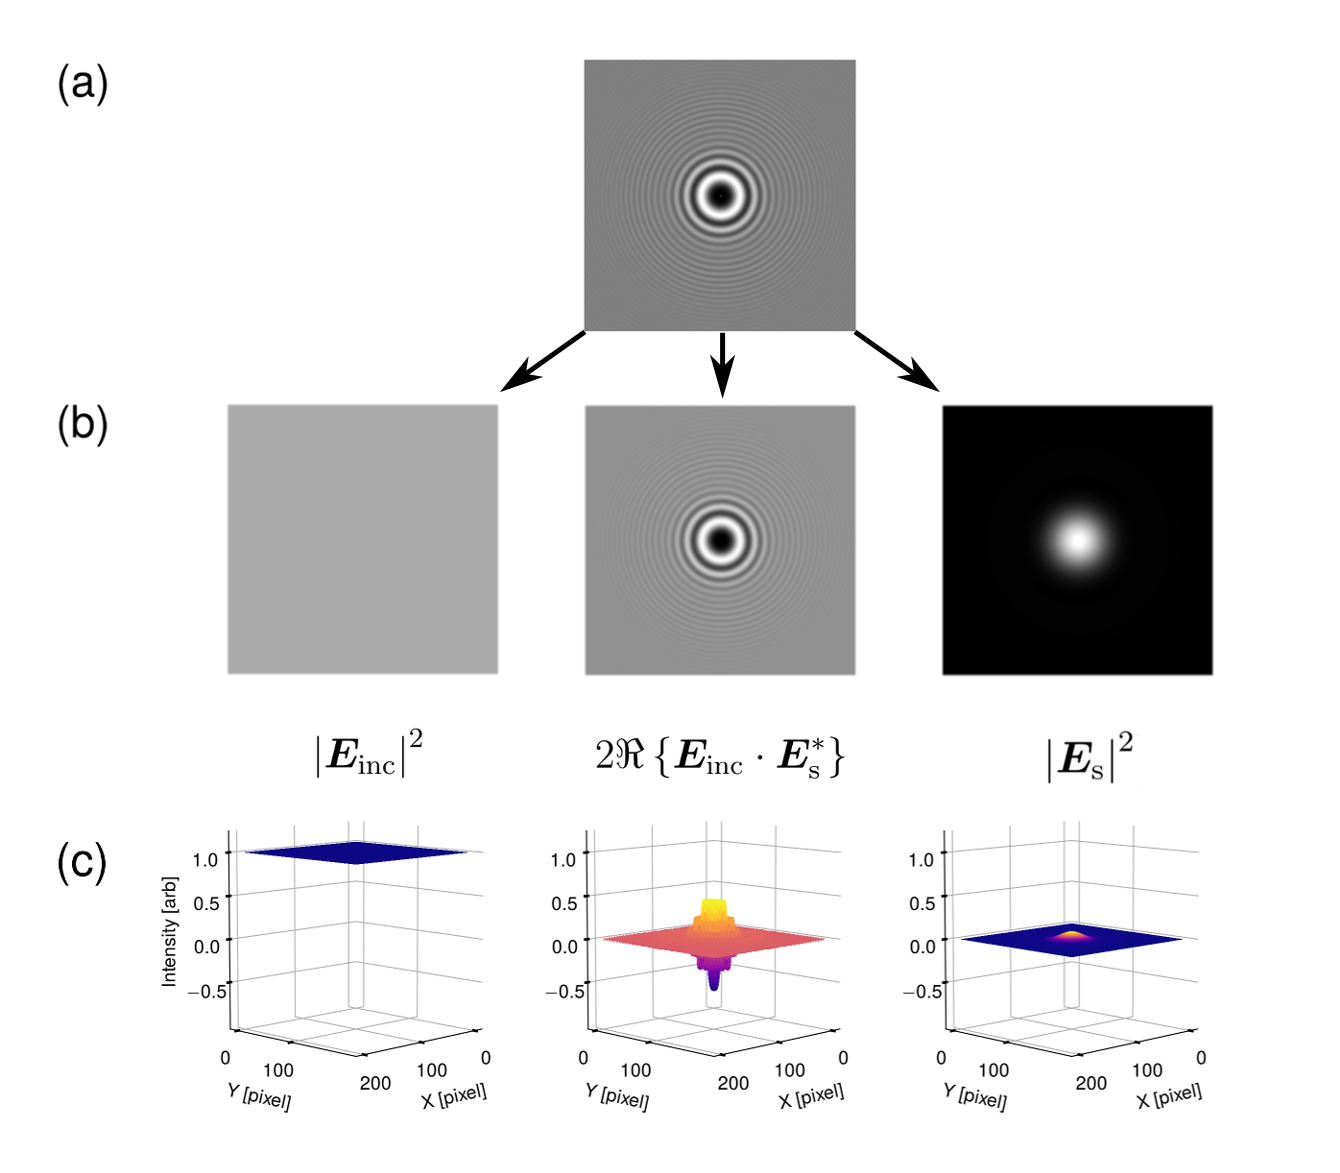
\includegraphics[width=\textwidth]{hvm_three_contributions}
  \caption{Depicting the three contributions to a holographic image. (a) the
    resulting intensity from a micron-sized scatterer above the focal plane.
    (b) The three contributions shown separately. (c) the magnitude of intensity
  for each term normalized by the intensity of the incident field.}
  \label{fig:three_contributions}
\end{figure}


\subsection{Scattering}
\label{ch:hvm:sec:hvm:ssec:scattering}

It is a general principle of linear, homogeneous media that the magnitude of the
scattered wave be proportional to the magnitude of the illuminating wave.
We therefore model the scattered field as

\begin{equation}
  \label{eq:incidentfield}
  \escat(\vec{r}) = E_0(\vec{r_p})\, \vec{f_s} \left ( k \left ( \vec{r} - \vec{r_p} \right ) \right ) ,
\end{equation}
where $E_0(\vec{r_p}$ is the average intensity illuminating the scatterer at $\vec{r_p}$,
and $\vec{f_s}$ describes how the particle $s$ scatters $\hat{x}$-polarized light.
Note that nature of $\vec{f_s}$ depends heavily on the shape and composition
of the scatterer.


With the exception of \autoref{ch:dimpled}, our study will
focus exclusively on spherical scatterers. 

%The Lorenz-Mie theory
%constitutes an exact solution for a plane wave scattering off of a
%dielectric sphere in a homogeneous medium.

\begin{equation}
\label{eq:scatteredfield}
  \vec{f}_s(k \vec{r}) = \sum_{n=1}^\infty \, f_n \, \left(
    i a_n \, \vec{N}^{(3)}_{e1n}(k \vec{r}) - b_n \,
    \vec{M}^{(3)}_{o1n}(k \vec{r})
    \right),
\end{equation}
where $f_n=i^n (2n+1)/[n(n+1)]$, and $\vec{M}^{(3)}_{o1n}(\vec{x})$ and 
$\vec{N}^{(3)}_{e1n}(\vec{x})$ are the vector spherical harmonics,x
\begin{equation}
    \vec{M}^{(3)}_{o1n}(\vec{x}) = \frac{\cos\phi}{\sin\theta} \,
  P^1_n(\cos\theta) \, j_n(x) \, \uvec{\theta}
  - \sin\phi \, \frac{dP^1_n(\cos\theta)}{d\theta} \, j_n(x) \, \uvec{\phi},
\end{equation}
and
\begin{multline}
  \vec{N}^{(3)}_{e1n}(\vec{x}) = n(n+1) \, \cos\phi
  \,P^1_n(\cos\theta) \, \frac{j_n(x)}{x} \, \uvec{r} \\
  + \cos\phi \, \frac{dP^1_n(\cos\theta)}{d\theta} \,
  \frac{1}{x} \frac{d}{dx}\left[x j_n(x)\right] \, \uvec{\theta} \\
  - \frac{\sin\phi}{\sin\theta} \, P^1_n(\cos\theta) \,
  \frac{1}{x}\frac{d}{dx}\left[x j_n(x)\right] \, \uvec{\phi}.
\end{multline}
Here, $P^1_n(\cos\theta)$ is the associated Legendre polynomial of the
first kind, and $j_n(kr)$ is the spherical Bessel function of the
first kind of order $n$.
The expansion coefficients in Eq.~(\ref{eq:scatteredfield}) are given
by \cite{bohren83}
\begin{equation}
  a_n = \frac{m^2 j_n(mka_p) \left[ka_p \, j_n(ka_p)\right]^\prime -
    j_n(ka_p) \left[mka_p \, j_n(mka)\right]^\prime}{
    m^2 j_n(mka_p) \left[ka_p \, h^{(1)}_n(ka_p)\right]^\prime -
    h^{(1)}_n(ka_p) \left[mka_p \, j_n(mka_p)\right]^\prime},
\end{equation}
and
\begin{equation}
\label{eq:bn}
  b_n = \frac{j_n(mka_p) \left[ka_p \, j_n(ka_p)\right]^\prime -
    j_n(ka_p) \left[mka_p \, j_n(m ka_p)\right]^\prime}{
    j_n(mka_p) \left[ka_p \, h^{(1)}_n(ka_p)\right]^\prime -
    h^{(1)}_n(ka_p) \left[mka_p \, j_n(mka_p)\right]^\prime},
\end{equation}

\subsection{Digital Recording}
\label{ch:hvm:sec:hvm:ssec:digitalrec}

% What are digital images. How are digital images recorded?
% Why are you telling them such things?
% How is it that digital images do not record intensity?

Images in science are ubiquitous; by sampling the intensity over an exposure
period, a single image encodes a bevy of spatial information that is ripe
for qualitative and quantitative analysis. Historically, researchers would
extract this information by hand. Jean-Perrin used a projector, pen and a paper to originally
measure the diffusion of a polymer bead. Crystallographers such as %FIXME: Add reference.
traced photographs of crystalline diffraction patterns by hand. Presently researchers utilize
digital cameras to record and digitize images as arrays of values. 

We utilize a digital camera to record holograms. To fit our experimental holograms to
theory and to simulate our digital recordings it is necessary to have a basic
understanding digital images. In this section we will 

\subsubsection{Digitizing Images}
\label{ch:hvm:sec:hvm:ssec:digitalrec:sssec:digitizing}

Modern digital cameras employ an array of photon detectors to measure the
average intensity over the sensor surface. Each photon detector, referred to as a pixel,
utilizes the photoelectric effect to convert photons into excited electrons.
The excited electrons at each pixel are counted, sometimes to single precision, and
then digitized into $8$-, $12$-, or even $16$-bit integers. Because the number of
excited electrons is proportional to the number of photons, and the the number of
photons is in turn proportional to the intensity of the of the image at the
sensor surface, the array of electron counts serves as a proxy for the intensity
of the image.

With millions of pixels and the capacity to count tens of thousands of electrons at each pixel,
digital cameras are an engineering marvel. For our purposes, we will review a few of the physical
details of a single pixel to explain important imaging effects such as dark counts, saturation,
and the digitization procedure.

Pixels are designed to accurately count the number of electrons that are
excited by incident photons within a given exposure period. A number of physical constraints
limit the accuracy of each pixels.

During an exposure period, $N_p$ photons of a particular wavelength arrive at a pixel
surface. Some fraction of the incident photons are converted to excited electrons
with a wavelength dependent probability known as the quantum efficiency. To be properly
counted, these excited electrons must survive until the counting procedure has
accounted for their presence. To this end, each pixel is doped to increase the lifetime
of excited electrons. In addition, the excited electrons must remain in the bulk so that
they are not grounded; for this purpose, a biased field is applied. % FIXME: What about mirror charges?

During the exposure period, a number of electrons can be thermally excited (as opposed to
photonically excited) and will be included in the count. These erroneously
counted electrons are referred to as a dark count. Measuring the average dark count of a
camera is as easy as recording the average image while an opaque object is blocking the
camera's sensor. Note that the dark count will increase with the length of the exposure
period.

% The number of electrons that can be negative.. scientific cameras have a non-zero
% floor to maintain gaussian-errors.
% Saturation occurs because the relation number of excited electrons per
% number of incident photons becomes non-linear. The largest number of reported
% electrons is the highest level

% A number of approximations come to mind with the LM theory.
% Approximation of radial component
% Approximation of functional form (Hankel function)
% Approximation of polarization


\section{Implementing Holographic Video Microscopy}

In this section we will describe the details of our microscope and
the experimental methods that were implemented in the ensuing chapters.



\subsection{Instrumentation}

We
% Illumination
% Objective
% Tube lens
% Camera


\subsection{Sample Preparation}

% Colloidal Synthesis.
% Flow Cells.
% Sealed Samples.



\subsection{Image Analysis}

% Normalization.
% Detecting and Localizing Features
% Fitting with Levinberg-Marquardt
% Mention Dimiduk's Bayesian analysis.

\subsection{Feature Detection}

After appropriately normalizing an image, it is necessary to detect if any holographic
features are in the field of view. 


\section{Applications of HVM}

% Broad uses exemplified in this thesis.
% Uses elsewhere
